% !TEX TS-program = xelatex
% !BIB program = bibtex
% !TEX encoding = UTF-8 Unicode

\documentclass[
  twoside,
  openany,                        % openright | openany
  degree    = master,               % degree = master | doctor
  language  = english,              % language = chinese | english
  fontset   = template,             % fontset = default | template | system | overleaf
  watermark = true,                 % watermark = true | false
  doi       = true,                 % doi = true | false
]{ntuthesis}

% !TeX root = ./main.tex

% --------------------------------------------------
% 資訊設定（Information Configs）
% --------------------------------------------------

\ntusetup{
  university*   = {National Taiwan University},
  university    = {國立臺灣大學},
  college       = {電機資訊學院},
  college*      = {Electrical Engineering and Computer Science},
  institute     = {電信工程學研究所},
  institute*    = {Graduate Institute of Communication Engineering College},
  title         = {上行非正交多重存取接收器之效能分析與基於調變編碼方式之使用者配對應用},
  title*        = {Performance Analysis of Uplink NOMA Receivers and Their Application to MCS-Based User Pairing},
  author        = {洪睿帆},
  author*       = {Jui-Fan Hung},
  ID            = {R13942124},
  advisor       = {林茂昭, 李世凱},
  advisor*      = {Mao-Chao Lin, Shih-Kai Lee},
  date          = {2026-07-28},         % 若註解掉，則預設為當天
  oral-date     = {2026-07-28},         % 若註解掉，則預設為當天
  DOI           = {10.5566/NTU2018XXXXX},
  keywords      = {非正交的多重存取接收器, 多資源功率域非正交的多重存取, 分增益多重存取, 調變編碼方式之使用者配對}, %關鍵字中文
  keywords*     = {NOMA rceiver, multi-resource PD-NOMA, GDMA, MCS user pairing}, %關鍵字英文
}

% --------------------------------------------------
% 加載套件（Include Packages）
% --------------------------------------------------

\usepackage[numbers,sort&compress]{natbib}      % 參考文獻
\usepackage{amsmath, amsthm, amssymb}   % 數學環境
\usepackage{amssymb, amsfonts, bm}

\usepackage{subcaption}
\usepackage{textcomp}
\usepackage{xcolor}
\usepackage{tikz}
\usepackage{physics} % 引入 physics 套件

\usepackage{algorithm}
\usepackage{algorithmic}
%\usepackage{algorithmicx}
%\usepackage{algpseudocode}

\usepackage{ulem, CJKulem}              % 下劃線、雙下劃線與波浪紋效果
\usepackage{booktabs}                   % 改善表格設置
\usepackage{multirow}                   % 合併儲存格
\usepackage{diagbox}                    % 插入表格反斜線
\usepackage{array}                      % 調整表格高度
\usepackage{longtable}                  % 支援跨頁長表格
\usepackage{paralist}                   % 列表環境


\usetikzlibrary{arrows.meta, shapes.geometric, calc}
\usepackage{booktabs}
\usepackage[table]{xcolor}
\usepackage{nicematrix}
\usepackage{makecell}

\usepackage{lipsum}                     % 英文亂字
\usepackage{zhlipsum}                   % 中文亂字
\usepackage{comment}
\usepackage{graphicx}
% --------------------------------------------------
% 套件設定（Packages Settings）
% --------------------------------------------------
\usetikzlibrary{positioning, arrows.meta, fit, calc, decorations.pathreplacing}


\begin{document}

% 封面與口試審定
% Cover and Verification Letter
\makecover                          % 論文封面（Cover）
\makeverification                   % 口試委員審定書（Verification Letter）

% 致謝與論文摘要
% Acknowledgement and Abstract
% !TeX root = ../main.tex

\begin{acknowledgement}

我愛Bubble姐, Latte哥, 齁齁齁, Tung姐姐，謝謝大家總是邀我打蘑菇，在我最脆弱的時候，當我想你你怎會淚流，當我想起你 怎會心痛 (想起你怎麼會心痛)
當你的心被牽走 牽的卻不再是我 當我難過 你跟著他走
當你說 還是朋友 (你說我們還是朋友) 我說 我還能說什麼
下過 ，大雨的午後 ，走過熟悉的你家門口
回憶湧上心頭 ，當時 ，純真的你和我

你總是狠狠吃定我 ，吃定我對你 ，愛的那麼多
多少次打勾勾 ，多少次我照做

你說 ，牽手可是 ，會把女生 ，的心牽走 ，我毫不猶豫的緊握
我說 ，能不能夠 ，能不能夠 ，讓時間停留 ，在你還沒放手的時候

\end{acknowledgement}       % 致謝（Acknowledgement）
% !TeX root = ../main.tex

\begin{abstract}

本論文針對上行非正交的多重存取（non-orthogonal multiple access, NOMA）系統進行比較分析。首先，在未編碼單一資源系統中，比較功率域非正交的多重存取（power-domain NOMA, PD-NOMA）與分增益多重存取（gain division multiple access, GDMA）的錯誤率表現。
接著將功率域非正交的多重存取 (PD-NOMA) 延伸至多資源系統模型，並在未編碼傳輸下比較 MMSE-SIC 偵測器與高密度簽名碼分
碼多重存取（high density signature CDMA, HDS-CDMA）的效能。

其次，本論文探討不同的編碼多資源 NOMA 接收器，並進一步將這些接收器延伸至正交分頻多工（orthogonal frequency division multiplexing, OFDM）架構下的 NOMA 系統。

最後，我們提出一個基於調變編碼方式（modulation coding scheme, MCS）的使用者配對架構，用以評估 NOMA 資源共享對系統層級頻譜效率（spectral efficiency, SE）表現的影響。

\end{abstract}

\begin{abstract*}

This thesis presents a comparative study of uplink non-orthogonal multiple access (NOMA) systems. 
First, uncoded single-resource power-domain NOMA (PD-NOMA) is compared with gain division multiple access (GDMA). PD-NOMA is then extended to a multi-resource model, where MMSE-SIC detection is evaluated against high density signature CDMA (HDS-CDMA) under uncoded transmission. 

Second, different coded multi-resource NOMA receivers are discussed. This receivers are further extended to orthogonal frequency division multiplexing (OFDM)-based NOMA systems.

Finally, a modulation coding scheme (MCS)-based user-pairing framework is developed to evaluate the system-level spectral efficiency (SE) behavior caused by NOMA resource sharing.

\end{abstract*}              % 摘要（Abstract）

% 生成目錄與符號列表
% Contents of Tables and Denotation 

%% 原本格式: 強制從奇數頁開始 %% 
% \maketableofcontents                % 目錄（Table of Contents）
% \makelistoffigures                  % 圖目錄（List of Figures）
% \makelistoftables                   % 表目錄（List of Tables）
%% 原本格式: 強制從奇數頁開始 %% 

%% 新格式 %%
% Remove blank pages inserted by \cleardoublepage in the front matter.
% The NTU thesis template uses \cleardoublepage for TOC/LOF/LOT and \mainmatter
% to force the next part to start on an odd page in two-sided printing.
% Here we temporarily replace it with \clearpage to keep these pages continuous.
\let\origcleardoublepage\cleardoublepage
\let\cleardoublepage\clearpage
\maketableofcontents
\makelistoffigures
\makelistoftables
%% 新格式 %%


% % !TeX root = ../main.tex

\begin{denotation}[3cm]
  \item[]       
\end{denotation}
            % 符號列表（Denotation）

% 論文內容
% Contents of Thesis
\mainmatter
\let\cleardoublepage\origcleardoublepage


% !TeX root = ../main.tex

\chapter{Introduction}


As the demand of high speed and low latency communication networks, future wireless systems must support higher spectral efficiency, flexible resource sharing, and massive connectivity. To increase the channel capacity and reliability, multiple access(MA) techniques become more important. 
It can be classified into two categories: Orthogonal multiple access (OMA) and non-orthogonal multiple access (NOMA).
There are many OMA techniques, such as time division multiple access in two generation (2G), Code Division Multiple Access (CDMA) in third generation (3G) and Orthogonal Frequency Division Multiple Access (OFDMA) in fourth generation (4G).~\cite{navita2016performance}
However, Orthogonal multiple access (OMA) avoids inter-user interference by assigning disjoint resources, its user capacity is fundamentally limited by the number of orthogonal resource units~\cite{dai2018survey}. 

In particular, beyond 5G and toward 6G, Non-Orthogonal multiple access (NOMA) is regarded as a potential multiple access technique to support the growing demands for massive connectivity and diverse service requirements.~\cite{clerckx2024multiple}.
In NOMA systems, multiple users are allowed to transmit over the same resource, relaxing the one-user-per-resource constraint and improving resource utilization at the cost of receiver-side interference management. 
Different NOMA schemes rely on different user-separation principles. For example, gain division multiple access (GDMA) separates users by exploiting their complex channel gains and is typically associated with joint MAP or ML detection \cite{hsu2019gain}. 
Power-domain NOMA (PD-NOMA) mainly relies on received-power disparity and usually adopts successive interference cancellation (SIC) \cite{islam2016power, dai2018survey}. 
Code-domain schemes such as SCMA, low density signature CDMA (LDS-CDMA) and HDS-CDMA exploit sparse or structured signatures for user separation\cite{nikopour2013sparse,lin2023gdma}. 
Pattern division multiple access (PDMA) maps users onto shared orthogonal resources according to a predefined pattern matrix~\cite{kong2016multiuser}.

In uplink NOMA, the base station (BS) receives the superimposed signals from multiple users and performs multiuser detection (MUD) to separate the users. That is, the receiver structure is often the key factor that determines both reliability and practicality.



% !TeX root = ../main.tex

\chapter{Single resource systems}
\label{ch:single-resource}
This chapter studies uplink NOMA with single resource system, where PD-NOMA with soft SIC and GDMA ~\cite{hsu2019gain} are discussed. 
We assume that the channel state information (CSI) is perfectly known at the receiver. The performance of these two detection schemes is evaluated in terms of bit error rate (BER) under different large scale fading coefficients.
\begin{comment}
Last, we clarify the performance gap between GDMA detection and soft SIC detection under different large scale fading coefficients.
\end{comment}

\begin{comment}
Last, we compare the bit error rate(BER) performance of this two detectors.
\end{comment}


\section{Single resource system model}
Consider an uplink system where perfect timing synchronization is assumed. $U$ users transmit simultaneously over one shared resource, which may be a frequency band, time slot, or spreading signature. The received signal at the BS is
\begin{equation}
    \label{eq:single_resource_system_model}
    y = \sum_{k=1}^{U} \sqrt{P_k \beta_k} h_k x_k + n,
\end{equation}
where $P_k$ is the transmit power of user $k$, $\beta_k$ is the large-scale fading coefficient of user $k$, $h_k$ is the small-scale Rayleigh flat-fading coefficient of user $k$, $x_k$ is transmission symbol of user $k$ and $n \sim \mathcal{CN}(0,N_0)$ is complex AWGN. 
Equivalently, the noise variance per dimension is $\sigma^2=N_0/2$. 
In this work, for simplicity, $P_k=1$ is assumed unless otherwise stated.

\section{Detection principle for PD NOMA : soft SIC}
\label{sec:Detection principle for PD NOMA : soft SIC}
In PD-NOMA, users are mainly separated by their received-power difference. The instantaneous received-power metric of user $k$ can be written as
\begin{equation}
    \rho_k = P_k\beta_k |h_k|^2 \triangleq |g_k|^2.
\end{equation}
The SIC detection order is denoted by
\begin{equation}
    \pi=\{\pi(1),\pi(2),\ldots,\pi(U)\},
\end{equation}
where $\pi(i)$ is the user detected at stage $i$. For received power-based ordering, this order is usually determined such that
    $\rho_{\pi(1)} \geq \rho_{\pi(2)} \geq \cdots \geq \rho_{\pi(U)}$.
The user indices are then relabeled according to this order.
For simplicity, we assume the user indices in \eqref{eq:single_resource_system_model} have been renumbered, so that the $i^{th}$ SIC stage detects the LLR of user $i$, denoted $L_{x_i}$.

At the first SIC stage, the LLR of $x_1$, $L_{x_1}$, is obtained by regarding signals from other users as approximately Gaussian in \eqref{eq:single_resource_system_model} and the soft estimate is denoted as $\hat{s}_{1}$.
At the $(i+1)^{th}$ SIC stage, the LLR of $x_{i+1}$, $L_{x_{i+1}}$, is obtained by a residual signal $y_{(i+1)}$ which is obtained by subtracting the contribution of the soft estimate $\hat{s}_{i}$ in the $i^{th}$ stage and regarding signals from other users as Gaussian. Therefore, 
\begin{equation}
    y_{(1)} = y,
\end{equation}
\begin{equation}
 \label{eq:subtract}
    y_{(i+1)}
    =
    y_{(i)}
    -
    g_{i}\hat{s}_{i}.
\end{equation}
For BPSK modulation, the log likelihood ratio (LLR) of user $i$ can be simplified as
\begin{equation}
    \label{eq:LLR}
    L_{x_i}
    =
    \log
    \frac{
    p(y_{(i)}|x_{\pi(i)}=+1)
    }{
    p(y_{(i)}|x_{\pi(i)}=-1)
    }
    =
    \frac{
    4\Re\{
    g_{i}^* y_{(i)}\}
    }{
    \sigma_{\mathrm{eff},(i)}^{2}
    }.
\end{equation}
The soft estimate of the detected symbol given $y_{(i)}$ is expressed ~\cite{shapiro2005soft} by
\begin{equation}
    \label{eq:soft calculation}
    \hat{s}_{i}
    =
    \mathbb{E}\left[x_{i}|L_{x_i}\right]
    =
    \tanh\left(\frac{L_{x_i} }{2}\right).
\end{equation}
and the conditional variance is obtained ~\cite{shapiro2005soft} as
\begin{equation}
    \label{eq:soft variance}
    \sigma^2_{\hat{s}_i}
    =
    \mathbb{E}\left[x^2_i|L_{x_i}\right]
    =
    1-\tanh^2 \left(\frac{L_{x_i}}{2}\right).
\end{equation}
Therefore, the effective noise variance is
\begin{equation}
    \sigma_{\mathrm{eff},{(i)}}^2
    =
    2\sigma^2
    +
    \sum_{j=i+1}^{U}
    |g_{j}|^2
    + 
    \sum_{j=1}^{i-1}
    \sigma^2_{\hat{s}_{j}}.
\end{equation}
The first term is the noise variance, the second term is the interference from undetected users, and the third term is the uncertain residual interference from previously detected users.
This procedure is repeated until all users are detected.

\section{Detection principle for GDMA}
\label{sec:Detection principle for GDMA}

In GDMA, users are distinguished by their distinct channel gains. Unlike PD-NOMA, which relies mainly on received-power differences, GDMA uses both the magnitude and phase of $g_k$.

\begin{table}[htbp]
        \centering
        \caption{Mapping rules for superimposed signal in the case of $M = 1$ and $U = 2$}
        \renewcommand{\arraystretch}{1.5} % 增�?每�??��?高度
        \setlength{\tabcolsep}{10pt}      % 增�?欄�?左右?��?
        \resizebox{1.15\width}{!}{
      \begin{tabular}{|c|c|c|c|c|c|}
        \hline
        $l$  & $x_1$ & $x_2$ & $s_l$ \\ \hline
        0 & 1 & 1 & $\sqrt{\beta_1}h_1 + \sqrt{\beta_2}h_2$ \\ \hline
        1 & 1 & -1 & $\sqrt{\beta_1}h_1 - \sqrt{\beta_2}h_2$ \\ \hline
        2 & -1 & 1 & $-\sqrt{\beta_1}h_1 + \sqrt{\beta_2}h_2$ \\ \hline
        3 & -1 & -1 & $-\sqrt{\beta_1}h_1 - \sqrt{\beta_2}h_2$ \\ \hline
      \end{tabular}
      }
      
      \label{table:superimposed-bpsk-u2}
\end{table}

At the receiver, the superimposed signal is first used to calculate the $a$ $posteriori$ probabilities (APPs) of all possible combinations of multiuser symbols, and then the LLR of each user is then obtained accordingly ~\cite{hsu2019gain}. There are $2^{MU}$ possible superimposed signal levels, denoted by the set
\begin{equation}
    \mathcal{S}
    =
    \{s_0,s_1,\ldots,s_{2^{MU}-1}\},
\end{equation}
where $M$ is the number of coded bits per modulation symbol for each user and $s_l\in\mathcal{S}$ contributes to the signal part in \eqref{eq:single_resource_system_model}. 
Take BPSK modulation ($M=1$) as an example, the superimposed signal 
\begin{equation}
  \begin{split}
    s_l &= (-1)^{l_2[1]} \cdot \sqrt{\beta_1}h_1 + (-1)^{l_2[2]} \cdot \sqrt{\beta_2}h_2 + \cdots + (-1)^{l_2[U]} \cdot \sqrt{\beta_U}h_U \\
    &= \sum_{k=1}^{U} (-1)^{l_2[k]} \cdot \sqrt{\beta_k}h_k, \quad l=0,1,\ldots,2^U-1,
  \end{split}
\end{equation}
where $l_2[k]$ denotes the transmission bit of user $k$ in the binary representation. 

In detail: 
\begin{equation}
  \begin{aligned}
    l=0 &\rightarrow (l_2[1], l_2[2], \ldots, l_2[U]) = (0, 0, \ldots, 0) \\
    l=1 &\rightarrow (l_2[1], l_2[2], \ldots, l_2[U]) = (0, 0, \ldots, 1) \\
    &\vdots \\
    l=2^U-1 &\rightarrow (l_2[1], l_2[2], \ldots, l_2[U]) = (1, 1, \ldots, 1).
  \end{aligned}
\end{equation}
The superimposed signal levels $s_l$ for the case $U=2$ are listed in Table~\ref{table:superimposed-bpsk-u2}, where $l \in \{0,1,2,3\}$.

The receiver computes the $a$ $posteriori$ probabilities (APPs) of each possible superimposed signal $s_l\in\mathcal{S}$ by
\begin{equation}
    P(s_l|y) = P(y|s_l) \cdot \frac{P(s=s_l)}{P(y)}. 
\end{equation}
Assuming the signals in $\mathcal{S}$ are equally probable, the APPs can be formulated as
\begin{equation}
    P(s_l|y)  \propto\exp\left(-\frac{|y-s_l|^2}{2\sigma^2}\right).
\end{equation}
The log-likelihood ratio (LLR) of user $k$ is then calculated by
\begin{equation}
    L_{x_k} =
    \log
    \frac{
    \sum\limits_{ {x_k}=+1}
    \exp\left(-\frac{|y-s_l|^2}{2\sigma^2}\right)
    }{
    \sum\limits_{ {x_k}=-1}
    \exp\left(-\frac{|y-s_l|^2}{2\sigma^2}\right)
    }.
\end{equation}

\section{Simulations of PD NOMA with soft SIC and GDMA}
The single-resource simulations use BPSK modulation for each user over independent Rayleigh flat-fading channels. 
Figure~\ref{fig:single-resource-ber-1-1}, 
~\ref{fig:single-resource-ber-1-0-1} and 
~\ref{fig:single-resource-ber-1-0-01} show the BER performance of two users with different large-scale fading coefficients $(\beta_1, \beta_2)$.
As the large-scale fading gap becomes larger, the soft SIC detection converges toward the performance of the GDMA detection, indicating that the received-power disparity provides a clearer detection order and reduces the ambiguity of early cancellation stages. However, it comes at the severe cost of user fairness ~\cite{ding2015impact}.

Figure~\ref{fig:single-resource-ber-1-0-1-0-01} shows the BER performance of three users with $(\beta_1, \beta_2, \beta_3)=(1,0.1,0.01)$.
The three-user result further clarifies the limitation of soft SIC detection. As the number of users increases, soft SIC becomes more susceptible to error propagation because each cancellation stage depends on the reliability of the previous user's soft estimates. In contrast, GDMA evaluates the APP of the superimposed signals and can therefore maintain favorable BER performance as the number of users increases ~\cite{lin2023uplink, Lin2024RandomAccess}. However, this performance advantage comes with an exponential growth cost with $U$.


\begin{figure}[htbp]
    \centering{
    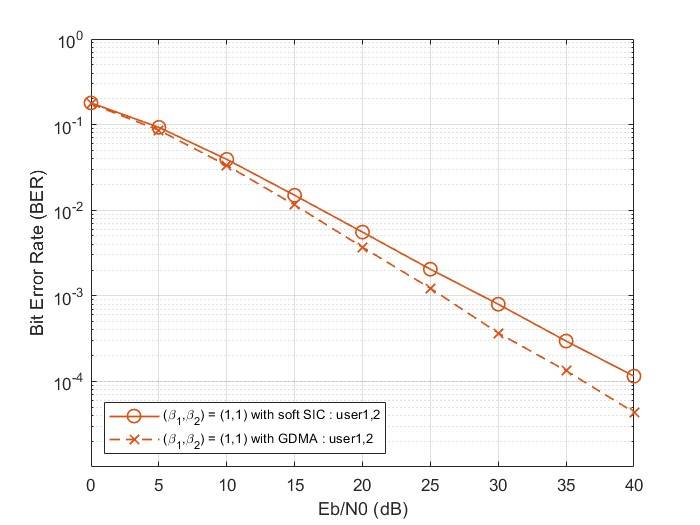
\includegraphics[width=0.9\linewidth]{figures/Chapter2/single_resource_beta1.jpg}}
    \caption{Users' BERs for single resource systems of $(\beta_1,\beta_2) = (1,1)$.}
    \label{fig:single-resource-ber-1-1}
\end{figure}
\begin{figure}[htbp]
    \centering
    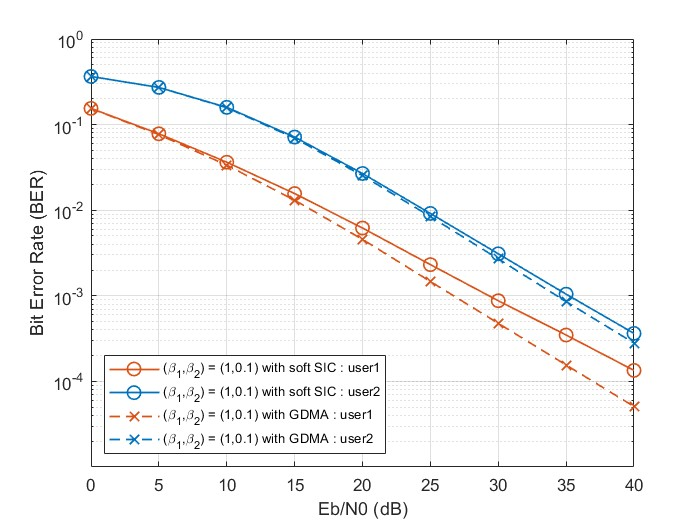
\includegraphics[width=0.9\linewidth]{figures/Chapter2/single_resource_beta0.1.jpg}
    \caption{Users' BERs for single resource systems of $(\beta_1,\beta_2) = (1,0.1)$.}
    \label{fig:single-resource-ber-1-0-1}
\end{figure}
\begin{figure}[htbp]
    \centering
    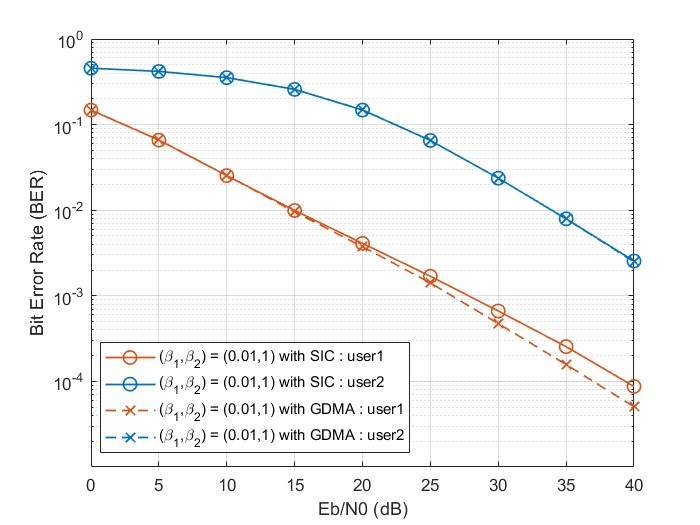
\includegraphics[width=0.9\linewidth]{figures/Chapter2/single_resource_beta0.01.jpg}
    \caption{Users' BERs for single resource systems of $(\beta_1,\beta_2) = (1,0.01)$.}
    \label{fig:single-resource-ber-1-0-01}
\end{figure}
\begin{figure}[htbp]
    \centering
    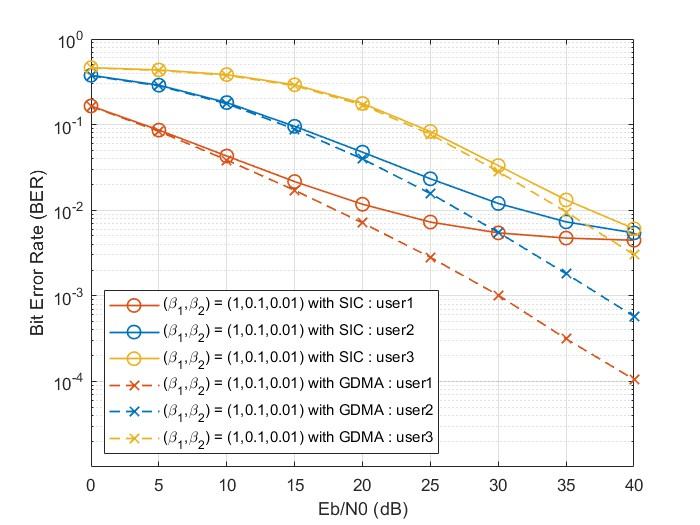
\includegraphics[width=0.9\linewidth]{figures/Chapter2/single_resource_beta0.1_U3.jpg}
    \caption{Users' BERs for single resource systems of $(\beta_1,\beta_2,\beta_3) = (1,0.1,0.01)$.}
    \label{fig:single-resource-ber-1-0-1-0-01}
\end{figure}






% !TeX root = ../main.tex

\chapter{Multiple resource NOMA systems}
\label{ch:multi-resource}
In this chapter, we extend single-resource PD-NOMA to a multiple-resource system, where several shared-resources are used to improve multiuser separation ability. 
Since single-resource PD-NOMA mainly relies on received-power differences, the multiple-resource model allows the BS to further exploit resource-domain channel-vector information. 
For multi-resource PD-NOMA, MMSE-SIC detection is adopted, post-SINR ordering and amplitude-based ordering are considered as two detection-ordering methods, and the performance is compared with HDS-CDMA with ML detection~\cite{lin2023gdma}.

\section{Multi-resource PD-NOMA system model}

Multi-resource PD-NOMA refers to an architecture in which each user can transmit over multiple shared resources. At one symbol time, the received vector is
\begin{equation}
    \bm{y} = \bm{H}\bm{x} + \bm{n},
    \label{eq:multi resource model}
\end{equation}
where $\bm{y}\in\mathbb{C}^{R\times 1}$ are the received signals over $R$ resources, $\bm{x}\in\mathbb{C}^{U\times 1}$ are the transmitted signals of $U$ users and $\bm{n}\in\mathbb{C}^{R\times 1}$ denotes complex AWGN. 
The channel matrix $\bm{H}\in\mathbb{C}^{R\times U}$ is 
\begin{equation}
    \bm{H}=
    \begin{bmatrix}
    \sqrt{P_1\beta_1}h_{1,1} & \sqrt{P_2\beta_2}h_{1,2} & \cdots & \sqrt{P_U\beta_U}h_{1,U}\\
    \sqrt{P_1\beta_1}h_{2,1} & \sqrt{P_2\beta_2}h_{2,2} & \cdots & \sqrt{P_U\beta_U}h_{2,U}\\
    \vdots & \vdots & \ddots & \vdots\\
    \sqrt{P_1\beta_1}h_{R,1} & \sqrt{P_2\beta_2}h_{R,2} & \cdots & \sqrt{P_U\beta_U}h_{R,U}
    \end{bmatrix}.
\end{equation}
The $k$th column $\bm{h}_k$ represents the resource-domain channel vector of user $k$.
For the representative two-resource and three-user case, the model is
\begin{equation}
    \begin{bmatrix}y_A\\y_B\end{bmatrix}
    =
    \begin{bmatrix}
    h_{A,1} & h_{A,2} & h_{A,3}\\
    h_{B,1} & h_{B,2} & h_{B,3}
    \end{bmatrix}
    \begin{bmatrix}x_1\\x_2\\x_3\end{bmatrix}
    +
    \begin{bmatrix}n_A\\n_B\end{bmatrix},
\end{equation}
where the large-scale fading and transmit-power factors are absorbed into each $h_{r,k}$.

We employ MMSE-SIC detection for \eqref{eq:multi resource model}. The resulting filter structure is similar to those widely used in multi-antenna systems~\cite{endo2012uplink,li2013advanced} and pattern division multiple access (PDMA) receivers~\cite{kong2016multiuser}. 
In multi-antenna reception, user separation mainly comes from spatial observations, while in PDMA it is further assisted by user-specific pattern mapping across resources. 
In contrast, the considered multi-resource PD-NOMA system does not adopt sparse signatures or pattern design\cite{mohammadkarimi2018signature}; instead, it relies on the channel vectors across shared resources to improve user separation reliability and overall performance. 
%Hence, our formulation should be interpreted as a resource-domain extension of PD-NOMA.


\section{MMSE-SIC Detection}
The MMSE-SIC receiver provides a low-complexity alternative to joint ML/MAP detection \cite{zanella2005mmse} by applying a linear MMSE filter and successively detecting and cancelling users.
The main quantities needed after filtering are the desired effective channel gain, the residual interference-plus-noise variance, the LLR, and the soft estimate used for cancellation.
For the multi-resource model of \eqref{eq:multi resource model}, 
consider user $k$ be detected. The MMSE filter is designed by following \cite[Eqs. (6), (7)]{kong2016multiuser} with the coefficient
\begin{equation}
\label{eq:coefficient}
    \bm{w}_k^H
    =
    \bm{h}_k^H
    \left(
    \bm{H}\bm{H}^H + 2\sigma^2\bm{I}
    \right)^{-1},
\end{equation}
The filter output of user $k$ can be formulated as
\begin{equation}
    \label{eq:filter output}
    z_k
    =
    \bm{w}_k^H \bm{y}
    =
    \bm{w}_k^H \bm{h}_k x_k
    +
    \sum_{j\neq k}\bm{w}_k^H \bm{h}_j x_j
    +
    \bm{w}_k^H \bm{n}.
\end{equation}
In \eqref{eq:filter output}, we define the effective channel gain:
\begin{equation}
    a_k=\bm{w}_k^H\bm{h}_k,
\end{equation}
and the effective residual interference-plus-noise variance:
\begin{equation}
	\label{eq:effective noise}
    \sigma_{k,\rm eff}^2
    =
    \sum_{j\neq k}
    |\bm{w}_k^H \bm{h}_j|^2
    +
    2\sigma^2 \|\bm{w}_k^H \|^2.
\end{equation}

\subsection{Detection Ordering}
\label{sec:MMSE SIC detection order}
To determine  successive detection orders in the SIC process, two ordering strategies are considered. The first is post-SINR ordering \cite{li2013advanced}. The post-filtering SINR of user \(k\) is
\begin{equation}
    \gamma^{\mathrm{post}}_k
    =
    \frac{\abs{\bm{w}_k^H\bm{h}_k}^2}
    {\sum_{j\ne k}\abs{\bm{w}_k^H\bm{h}_j}^2+2\sigma^2\norm{\bm{w}_k}^2}.
    \label{eq:post-sinr}
\end{equation}
The receiver detects the user with the largest post-SINR first. This criterion uses both the magnitude and phase of the channel information, and it reflects the actual quality of each user after MMSE filtering, which are generally preferred in reducing SIC error propagation.

The second strategy is amplitude-based ordering. Users are sorted according to a channel magnitude or received-power metric such as
\begin{equation}
    \gamma^{\mathrm{amp}}_k=\norm{\bm{h}_k}^2.
\end{equation}
This ordering is simpler because it relies only on channel magnitudes, but ignores how MMSE filtering suppresses multiuser interference.
After determining the SIC orders and then re-numbering the user indexes, we assume 
\begin{equation}
    \label{eq:detection order}
    \gamma_1 \geq \ldots \geq \gamma_U
\end{equation}
for simplicity.
This renumbering is applied for either one of the ordering strategies and simplifies the superscript.


\begin{comment}
\subsection{SIC Procedure}
After the order is chosen, users are renumbered as $1,2,\ldots,U$. The SIC procedure is similar to section ~\ref{sec:Detection principle for PD NOMA : soft SIC}. 
At the ${(i+1)}^{th}$ SIC stage, the SIC detector performs the subtraction by setting
\begin{equation}
    \label{eq:soft cancellation}
    \bm{y}_{(i+1)} = \bm{y}_{(i)} - \bm{h}_i \hat{s}_i
\end{equation}
with $\bm{y}_{(1)} = \bm{y}$, where $\bm{y}_{(i)}$ denotes the residual vector at stage $i$.
The corresponding column of $\bm{H}$ in \eqref{eq:multi resource model} is then removed by setting
\begin{equation}
    \bm{H}_{(i+1)}=[\bm{h}_{i+1},\ldots,\bm{h}_U]
\end{equation}
where $\bm{H}_{(1)} = \bm{H}$.
The process then goes back to re-calculate the coefficient $\bm{w}_{i+1}^H$ by using \eqref{eq:coefficient}, the corresponding filter output and the effective variance of the residual interferences and noise can be derived as 
\begin{equation}
    \label{eq:filter output stage i}
    z_{i}
    =
    \bm{w}_{i}^H \bm{y}_{(i)}
    =
    \bm{w}_{i}^H \bm{h}_{i} x_{i}
    +
    \sum_{j > i} \bm{w}_{i}^H \bm{h}_j x_j
    +
    \bm{w}_{i}^H \bm{n}.
\end{equation}
\begin{equation}
	\label{eq:effective noise stage i}
    \sigma_{i,\rm eff}^2
    =
    \sum_{j > i}
    |\bm{w}_{i}^H \bm{h}_j|^2
    +
    2\sigma^2 \|\bm{w}_{i}^H \|^2.
\end{equation}
For a general modulation alphabet $\mathcal{S}$, the LLR of the $q$th bit\cite{shapiro2005soft} is calculated by
\begin{equation}
    L_{x_i,q}
    =
    \log
    \frac{
    \sum\limits_{s\in\mathcal{S}_{q,+}}
    \exp\left(-\frac{\abs{z_i-a_i s}^2}{\sigma^2_{i,\mathrm{eff}}}\right)}
    {\sum\limits_{s\in\mathcal{S}_{q,-}}
    \exp\left(-\frac{\abs{z_i-a_i s}^2}{\sigma^2_{i,\mathrm{eff}}}\right)},
    \label{eq:mmse-sic-general-llr}
\end{equation}
where $\mathcal{S}_{q,+}$ and $\mathcal{S}_{q,-}$ are the subsets of constellation symbols whose $q$th bit is mapped to $+1$ and $-1$, respectively. 
The corresponding soft estimate \cite{shapiro2005soft}
\begin{equation}
    \hat{s}_i
    =
    \mathbb{E}[x_i|z_i]
    \approx
    \frac{
    \sum\limits_{s\in\mathcal{S}} s
    \exp\left(-\frac{\abs{z_i-a_i s}^2}{\sigma^2_{i,\mathrm{eff}}}\right)}
    {
    \sum\limits_{s\in\mathcal{S}}
    \exp\left(-\frac{\abs{z_i-a_i s}^2}{\sigma^2_{i,\mathrm{eff}}}\right)}.
    \label{eq:mmse-sic-general-soft-estimate}
\end{equation}
For BPSK modulation, $\mathcal{S}=\{+1,-1\}$, and \eqref{eq:mmse-sic-general-llr} becomes
\begin{equation}
    L_i
    =
    \frac{4\Re\{a_i^* z_i\}}{\sigma^2_{i,\mathrm{eff}}}.
\end{equation}


If $\hat{s}_i$ is unreliable, the subtraction leaves a cancellation residual in $\bm{y}^{(i+1)}$. This residual is one of the main sources of error propagation in MMSE-SIC, and it motivates the variance-aware coded receiver developed in Chapter~\ref{ch:coded}.
\end{comment}


\subsection{SIC Procedure}

After the order is decided, users are renumbered as $1,2,\ldots,U$. At stage $i$, the residual vector is $\bm{y}_{(i)}$ and the corresponding channel matrix is
\begin{equation}
    \label{eq:downsized channel matrix}
    \bm{H}_{(i)}=[\bm{h}_i,\bm{h}_{i+1},\ldots,\bm{h}_U].
\end{equation}
The MMSE filter output and the effective variance of the residual interferences and noise can be derived as 
\begin{equation}
    \label{eq:filter output stage i}
    z_{i}
    =
    \bm{w}_{i}^H \bm{y}_{(i)}
    =
    \bm{w}_{i}^H \bm{h}_{i} x_{i}
    +
    \sum_{j > i} \bm{w}_{i}^H \bm{h}_j x_j
    +
    \bm{w}_{i}^H \bm{n}.
\end{equation}
\begin{equation}
	\label{eq:effective noise stage i}
    \sigma_{i,\rm eff}^2
    =
    \sum_{j > i}
    |\bm{w}_{i}^H \bm{h}_j|^2
    +
    2\sigma^2 \|\bm{w}_{i}^H \|^2.
\end{equation}
After MMSE filtering, the output can be approximated as an equivalent scalar channel
\begin{equation}
    z_i = a_i x_i+\eta_i,
    \qquad
    a_i=\bm{w}_i^H\bm{h}_i,
    \qquad
    \eta_i\sim\mathcal{CN}(0,\sigma^2_{i,\mathrm{eff}}).
    \label{eq:mmse-sic-equivalent-scalar-channel}
\end{equation}
For a general bit-labeled constellation alphabet $\mathcal{S}$, let
$b_m(s)\in\{0,1\}$ denote the $m$th label bit of symbol $s$, and define
\begin{equation}
    \mathcal{S}_{m,b}
    =
    \{s\in\mathcal{S}: b_m(s)=b\},
    \qquad b\in\{0,1\}.
\end{equation}
In this chapter, the transmitted coded bits are assumed to be independent and equally probable. Therefore, the prior term cancels in the likelihood function. Under the scalar Gaussian approximation in \eqref{eq:mmse-sic-equivalent-scalar-channel}, the standard likelihood-marginalization form of the soft-output demapper~\cite{shapiro2005soft} gives the detector LLR of the $m$th bit as
\begin{equation}
    L_{x_i,m}
    =
    \log
    \frac{
    \sum\limits_{s\in\mathcal{S}_{m,0}}
    \exp\left(-\frac{\abs{z_i-a_i s}^2}{\sigma^2_{i,\mathrm{eff}}}\right)}
    {\sum\limits_{s\in\mathcal{S}_{m,1}}
    \exp\left(-\frac{\abs{z_i-a_i s}^2}{\sigma^2_{i,\mathrm{eff}}}\right)},
    \label{eq:mmse-sic-general-llr}
\end{equation}
For BPSK modulation, $\mathcal{S}=\{+1,-1\}$ with $0\mapsto +1$ and $1\mapsto -1$, and \eqref{eq:mmse-sic-general-llr} becomes
\begin{equation}
    L_{x_i}
    =
    \frac{4\Re\{a_i^* z_i\}}{\sigma^2_{i,\mathrm{eff}}}.
\end{equation}
The corresponding soft symbol estimate is the posterior mean obtained from the same equally likely symbol prior~\cite{shapiro2005soft}:
\begin{equation}
    \hat{s}_i
    =
    \mathbb{E}[x_i|z_i]
    =
    \frac{
    \sum\limits_{s\in\mathcal{S}} s
    \exp\left(-\frac{\abs{z_i-a_i s}^2}{\sigma^2_{i,\mathrm{eff}}}\right)}
    {
    \sum\limits_{s\in\mathcal{S}}
    \exp\left(-\frac{\abs{z_i-a_i s}^2}{\sigma^2_{i,\mathrm{eff}}}\right)}.
    \label{eq:mmse-sic-general-soft-estimate}
\end{equation}
This posterior mean reduces to

\begin{equation}
\hat{s}_i=\tanh(L_{x_i}/2)
\end{equation}
if BPSK modulation is used. 
The expression in \eqref{eq:mmse-sic-general-soft-estimate} is therefore a detector-output soft estimate for the uncoded receiver when all transmitted bits are equally likely. 
The soft estimate is then subtracted from the received vector:
\begin{equation}
    \bm{y}_{(i+1)}=\bm{y}_{(i)}-\bm{h}_i\hat{s}_i .
\end{equation}
The process then goes back to re-calculate the coefficient $\bm{w}_{i+1}^H$ by using \eqref{eq:coefficient} with $\bm{H}_{(i+1)}$. The LLR of $x_{i+1}$ and its soft estimate $\hat{s}_{i+1}$ can also be obtained by \eqref{eq:mmse-sic-general-llr} and \eqref{eq:mmse-sic-general-soft-estimate}. This procedure is repeated until all users are detected.

If $\hat{s}_i$ is unreliable, the subtraction leaves a residual of cancellation  in $\bm{y}_{(i+1)}$. This residual is the main source of error propagation in MMSE-SIC, and motivates the variance-aware coded receiver discussed in Chapter~\ref{ch:coded}.

\section{Uncoded Simulation Results}

The main uncoded multi-resource setting uses BPSK transmission, $R=2$ resources, $U=3$ users, independent Rayleigh flat fading, and perfect CSI are assumed. The MMSE-SIC detector is compared with HDS-CDMA with ML detection\cite{lin2023gdma}. We consider two large-scale fading cases: $(\beta_1,\beta_2,\beta_3)=(1,0.1,0.01)$ and $(\beta_1,\beta_2,\beta_3)=(1,1,1).$
$\bar{E}_b$ in the simulations represent the average transmit energy per bit per user, normalized by the number of resources.


\begin{figure}[htbp]
    \centering
    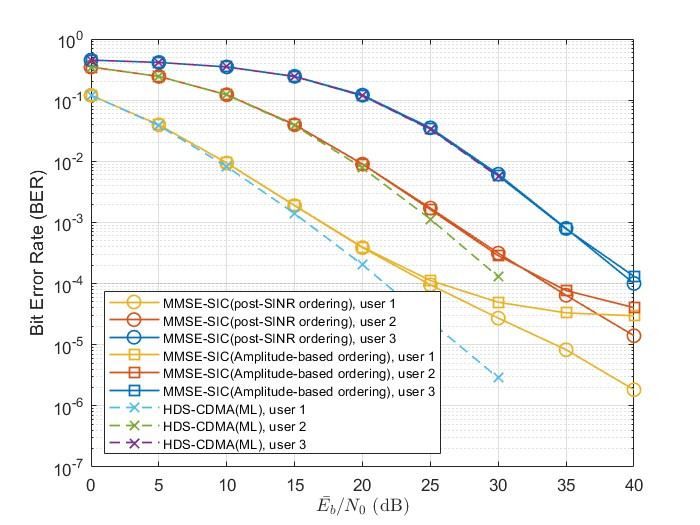
\includegraphics[width=0.9\linewidth]{figures/Chapter3/multi_resource_beta0.1.jpg}
    \caption{Multi-resource system. BER of MMSE-SIC and HDS-CDMA with ML detection with $R=2$, $U=3$ and $(\beta_1, \beta_2, \beta_3) = (1,0.1,0.01)$.}
    \label{fig:multi-resource-beta0-1}
\end{figure}
\begin{figure}[htbp]
    \centering
    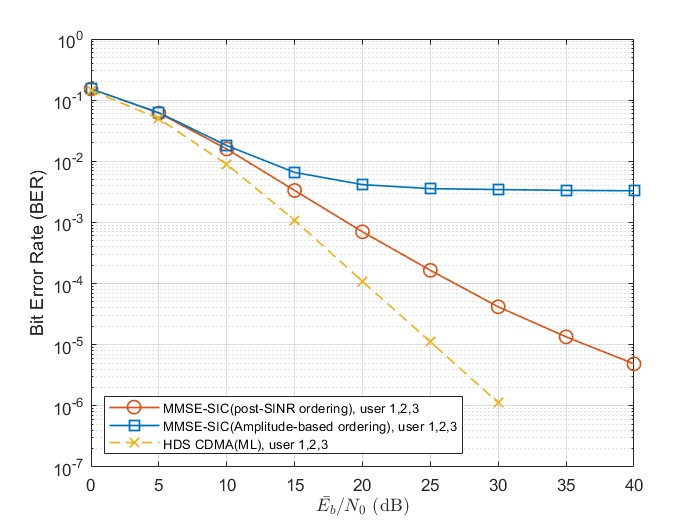
\includegraphics[width=0.9\linewidth]{figures/Chapter3/multi_resource_beta1.jpg}
    \caption{Multi-resource system. BER of MMSE-SIC and HDS-CDMA with ML detection with $R=2$, $U=3$ and $(\beta_1, \beta_2, \beta_3) = (1,1,1)$.}
    \label{fig:multi-resource-beta1}
\end{figure}

The results in figure.~\ref{fig:multi-resource-beta0-1} and \ref{fig:multi-resource-beta1} show that HDS-CDMA with ML detection achieves better uncoded BER than MMSE-SIC in both large-scale fading cases. For the unequal-$\beta_k$ case in figure.~\ref{fig:multi-resource-beta0-1}, HDS-CDMA performs about $3$ dB better than MMSE-SIC at $\mathrm{BER}=10^{-4}$ for user 1. For the equal-$\beta_k$ case in figure.~\ref{fig:multi-resource-beta1}, HDS-CDMA performs about $7$ dB better than MMSE-SIC at $\mathrm{BER}=10^{-4}$. 
Therefore, the performance loss of MMSE-SIC is much more significant when the users have similar average received powers.

The smaller BER gap of two detector in the unequal-fading case is caused by the large-scale fading disparity. Since the users have clearly separated average received powers, the first SIC stage is more reliable and the cancellation error is less likely to dominate the following stages. 
In particular, for the user with the smallest average received power, MMSE-SIC is close to HDS-CDMA within the simulated SNR range. 

The detection ordering comparison further explains the behavior of MMSE-SIC. In the unequal-$\beta_k$ case, amplitude-based ordering only causes a slight degradation around $25$ dB for user 1. In the equal-$\beta_k$ case, however, amplitude-based ordering degrades heavily.

These results indicate that multi-resource PD-NOMA improves user separation compared with single-resource soft SIC, but HDS-CDMA with ML detection remains the stronger uncoded benchmark. The residual performance gap thus motivates the coded system considered in the next chapter.

\begin{comment}
Chapter~\ref{ch:coded} introduces channel coding and iterative detection and decoder (IDD) so that the reliability of the decoder can be used to reduce the propagation of SIC errors.
\end{comment}



% !TeX root = ../main.tex

\chapter{Coded Multi-Resource Systems with IDD}
\label{ch:coded}

This chapter introduces channel coding and iterative detection and decoding (IDD) into the multi-resource receiver. Motivated by the error-propagation problem observed in uncoded SIC receivers, the detector exchanges soft information with the FEC decoder and refines interference cancellation through iterations based on a priori information update. 
The block error rate (BLER) performance gap of MMSE-SIC-IDD, MMSE-PIC-IDD and MAP-IDD are clarified in coded multi-resource uplink NOMA system.
\begin{comment}
This chapter develops MMSE-SIC-IDD and compares it with MMSE-PIC-IDD and MAP-IDD to clarify the performance gap in coded multi-resource uplink NOMA system.
\end{comment}

\section{Introduction of IDD structure}
For coded systems, the detector is typically embedded in an iterative detection and decoding (IDD) receiver. In this structure, soft information is exchanged between the detector and the FEC decoder \cite{uchoa2015iterative,studer2011asic,li2024low}. The detector produces bit-level LLRs for the coded bits, while the decoder uses the code constraints to refine the reliability information and returns updated soft information to the detector, which is the a priori information of next detector calculation. 
In our simulations, the IDD receiver is implemented with a maximum number of iterations $t_{\max}$, and the final decoder output is used to make hard decisions on the transmitted bits. 

\begin{figure}
    \centering
    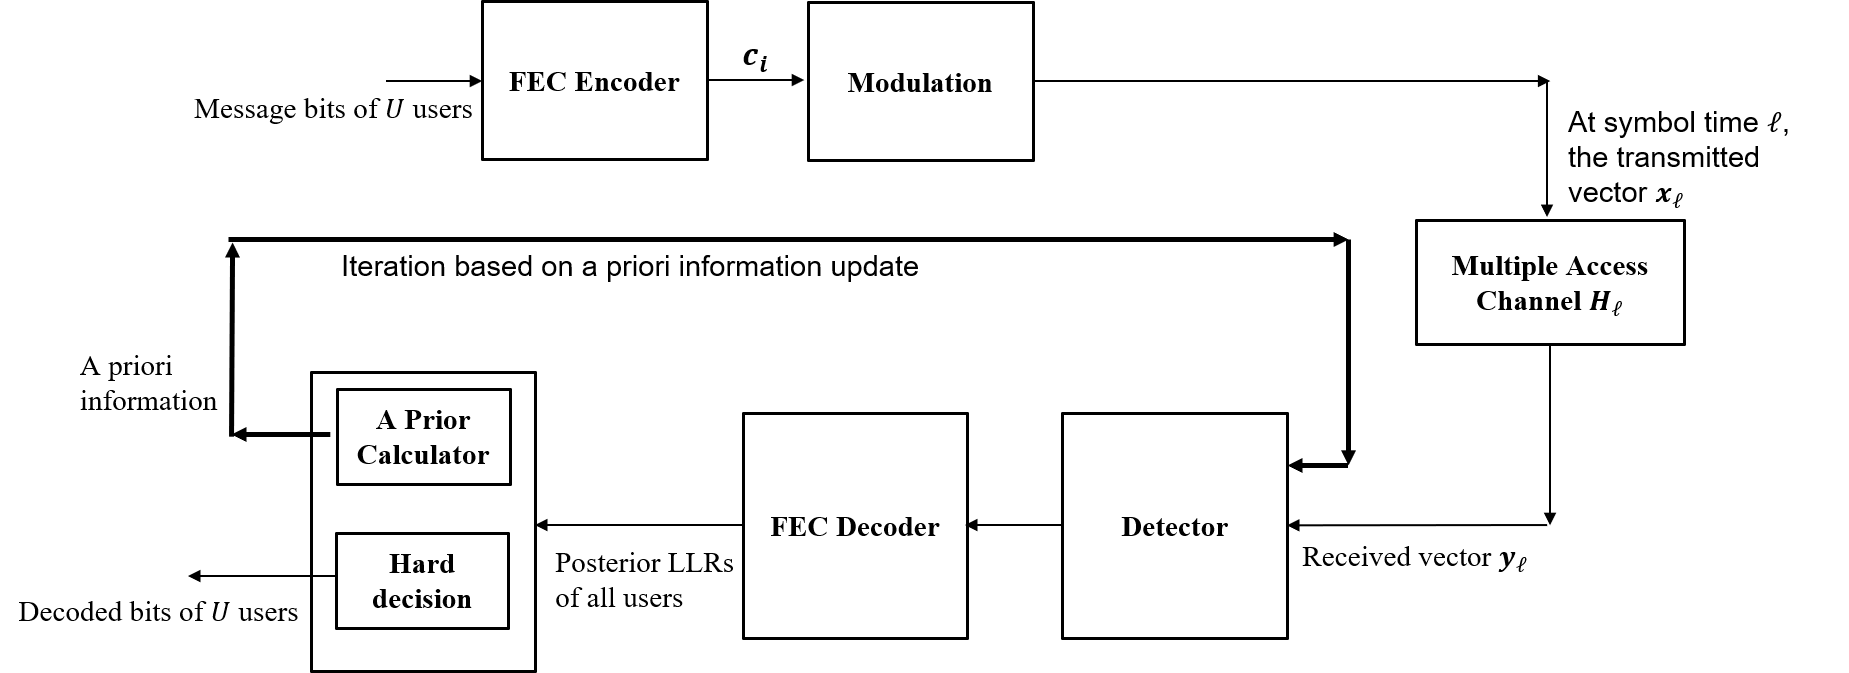
\includegraphics[width=0.9\linewidth]{figures/Chapter4/IDD_structure.png}
    \caption{Coded NOMA system with IDD receiver}
    \label{fig:IDD_structure}
\end{figure}

\section{Coded Multi-resource system model}
In this chapter, different users are allowed to employ different modulation schemes and different channel code lengths.
Let $\bm{c}_i$ denote user $i's$ transmitted codeword of length $N_{c,i}$
\begin{equation}
    \bm{c}_i=[c_{i,1},c_{i,2},\ldots,c_{i,N_{c,i}}]^T,
\end{equation}
After modulation, the codeword is grouped into $N_{s}$ modulation symbols. At symbol time $\ell$, the transmitted vector is
\begin{equation}
    \bm{x}_\ell=[x_{1,\ell},x_{2,\ell},\ldots,x_{U,\ell}]^T,
\end{equation}
Refer to equation \eqref{eq:multi resource model}, the received vector is
\begin{equation}
    \bm{y}_\ell=\bm{H}_\ell\bm{x}_\ell+\bm{n}_\ell.
    \label{eq:coded-symbol-model}
\end{equation}
In the block-fading simulations, $\bm{H}_1=\bm{H}_2=\cdots=\bm{H}_{N_s}$. For simplicity, we omit the subscript $\ell$, which denotes the process is dealing with $\bm{y_\ell}$. 
The overall block diagram of coded NOMA system with IDD receiver is shown in figure.~\ref{fig:IDD_structure}.

\section{MMSE-SIC-IDD}

In this section, we introduce the procedure of the MMSE-SIC-IDD receiver. The key feature of the structure is that interference cancellation in the SIC process is performed after channel decoding rather than immediately after detection.

\subsection{Receiver Procedure}
Following a similar procedure in section \ref{sec:MMSE SIC detection order}, the detection order can be obtained. For post-SINR ordering method, the additional $\bar{v}_i^{(t)}$ is considered and will be disscussed in section \ref{sec:Variance-Aware MMSE Filtering}. Assume the users are re-numbered from $1$ to $U$ according to this order. 

For user $i$, the detector first computes the bit-level LLRs $\bm{L}_{\bm{c}_i}$. The summation of these LLRs and a priori information are then passed to the FEC decoder of user $i$. After decoding, the decoder produces the a posteriori LLRs $\bm{L}^d_{\bm{c}_i}$, which are used to generate the decoded soft symbol estimate $\hat{\bm{s}}^d_i$. This decoded soft symbol estimate is then fed back to the MMSE-SIC detector for the next SIC stage, i.e., user $i+1$, where it is used to subtract the interference caused by user $i$. 
Intuitively, performing cancellation after decoding can improve the reliability of the cancelled signal and thus reduce error propagation in the SIC process.

Due to the successive decoding procedure, the extrinsic information of each user is collected asynchronously. Specifically, after decoding user $i$, the extrinsic LLRs are obtained as
\begin{equation}
    \label{eq:extrinsic LLR for next a priori update}
    \bm{L}^e_{\bm{c}_i} = \bm{L}^d_{\bm{c}_i} - \bm{L}^{in}_{\bm{c}_i},
\end{equation}
where $\bm{L}^{in}_{\bm{c}_i}$ is the input of decoder.
In this way, the decoded extrinsic information of all users is provided as a priori information to the MMSE-SIC detector in the following IDD iteration.

\subsection{Soft Information for a priori update}
\label{sec:Soft Information for a priori update}
Let $\mathcal{S}_i$ denote the modulation alphabet of user $i$, and let
$M_i=\log_2|\mathcal{S}_i|$ be the number of coded bits per modulation symbol. For a symbol
$s\in\mathcal{S}_i$, its binary label is written as
\begin{equation}
    \bm{b}_i(s)
    =
    [b_{i,0}(s),b_{i,1}(s),\ldots,b_{i,M_i-1}(s)] .
\end{equation}
Let $L^{(t)}_{c_{i},\ell,m}$ denote the a priori LLR of the $m$th coded bit in the $\ell$th modulation symbol of user $i$ at a priori update iteration $t$, with
\begin{equation}
    \label{eq:a priori LLR}
    L^{(t)}_{c_{i},\ell,m}
    =
    \log
    \frac{P^{a,(t)}(b_{i,\ell,m}=0)}
    {P^{a,(t)}(b_{i,\ell,m}=1)},
    \qquad
    L^{(0)}_{c_{i},\ell,m} = 0.
\end{equation}
The corresponding bit probability is
\begin{equation}
    P^{a,(t)}(b_{i,\ell,m}=b)
    =
    \frac{1}
    {1+\exp\left[-(1-2b)L^{(t)}_{c_{i},\ell,m}\right]},
    \qquad b\in\{0,1\}.
    \label{eq:bit-prior-from-llr}
\end{equation}
Assuming the interleaved coded bits are represented by independent bit priors at the demapper input, the a priori symbol probability is the product of its corresponding a priori bit probability\cite{tuchler2002minimum}, which is written as
\begin{equation}
    P^{a,(t)}_{i,\ell}(s)
    =
    \prod_{m=0}^{M_i-1}
    P^{a,(t)}(b_{i,\ell,m}=b_{i,m}(s)).
    \label{eq:symbol-prior-from-bit-priors}
\end{equation}
The soft symbol mean used for a priori update before detection is calculated according to the a priori symbol probability\cite{shapiro2005soft}, that is, 
\begin{equation}
    \mu^{(t)}_{i,\ell}
    =
    \mathbb{E}[x_{i,\ell}\mid \bm{L}^{(t)}_{c_{i},\ell}]
    =
    \frac{
    \sum\limits_{s\in\mathcal{S}_i}
    s P^{a,(t)}_{i,\ell}(s)}
    {\sum\limits_{s\in\mathcal{S}_i}
    P^{a,(t)}_{i,\ell}(s)} ,
    \label{eq:idd-general-soft-mean}
\end{equation}
and the corresponding symbol variance is
\begin{equation}
    \sigma^{2~(t)}_{i,\ell}
    =
    \frac{
    \sum\limits_{s\in\mathcal{S}_i}
    \abs{s}^2 P^{a,(t)}_{i,\ell}(s)}
    {\sum\limits_{s\in\mathcal{S}_i}
    P^{a,(t)}_{i,\ell}(s)}
    -
    \abs{\mu^{(t)}_{i,\ell}}^2 .
    \label{eq:idd-general-soft-var}
\end{equation}
For BPSK modulation with $0\mapsto +1$ and $1\mapsto -1$, equation \eqref{eq:idd-general-soft-mean} and \eqref{eq:idd-general-soft-var} reduce to
\begin{equation}
    \mu^{(t)}_{i,\ell}
    =
    \tanh\left(\frac{L^{(t)}_{c_{i},\ell,0}}{2}\right),
    \qquad
    \sigma^{2~(t)}_{i,\ell}
    =
    1-\abs{\mu^{(t)}_{i,\ell}}^2 .
\end{equation}
For simplicity, we consider the average variance of user $i$ over the coded block,that is,
\begin{equation}
    \label{eq:average variance of user i}
    \bar{v}^{(t)}_{i}
    =
    \frac{1}{N_s}\sum_{\ell=1}^{N_s}\sigma^{2~(t)}_{i,\ell},
\end{equation}
The variance matrix is defined as
\begin{comment}
To simplify the expression in the following equations, for the current a priori update $t$, we omit the update superscript in the variance matrix and rewrite it as
\end{comment}
\begin{equation}
    \bm{V}
    =
    \operatorname{diag}(\bar{v}_1^{(t)},\bar{v}_2^{(t)},\ldots,\bar{v}_U^{(t)}),
    \qquad
    \bar{v}_i^{(t)}>0.
    \label{eq:variance-matrix}
\end{equation}

When decoder feedback is reliable, $\bar{v}_i^{(t)}$ becomes small, indicating a higher probability of successful decoding for user \(i\) and consequently a smaller residual interference. 
Conversely, when decoder feedback is uncertain, he variance remains large, allowing the receiver to avoid overconfident cancellation.

\subsection{Variance-Aware MMSE Filtering}
\label{sec:Variance-Aware MMSE Filtering}
When all users' extrinsic information from the FEC decoder has been asynchronously collected, the variance-aware MMSE filter of user $k$ \cite[Eqs. (6), (7)]{studer2011asic} for next a priori based iteration can proceed with the coefficient
\begin{equation}
    \label{eq:variance-aware-mmse}
    \tilde{\bm{w}}^H_k
    =
    \bar{v}_k^{(t)}\bm{h}_k^H
    \left(
    \bm{H}\bm{V}\bm{H}^H + 2\sigma^2\bm{I}
    \right)^{-1}.
\end{equation}
the corresponding post-SINR can be written as 
\begin{equation}
    \label{eq:post-sinr-with-variance}
    \gamma^{\mathrm{post}}_k
    =
    \frac{\abs{\tilde{\bm{w}}^H_k\bm{h}_k}^2}
    {\sum_{j\ne k}\bar{v}_j^{(t)}\abs{\tilde{\bm{w}}^H_k\bm{h}_j}^2+2\sigma^2\norm{\tilde{\bm{w}}_k}^2}.
\end{equation}
Compared with equation \eqref{eq:coefficient} and \eqref{eq:post-sinr}, users with reliable a priori information contribute less uncertainty to the MMSE filtering process and SIC detection ordering.

\subsection{Decoder-Aided SIC Cancellation}

To simplify the expression in the following equations, we omit the subscript $\ell$, which denotes that the process is dealing with $\bm{y}_{\ell}$. The procedure goes back to MMSE-SIC stage 1, user 1 can benefit from the a priori information of users $2,\ldots,U$ by using
\begin{equation}
    \label{eq:idd-stage-one-residual}
    \bm{y}_{(1)}^{(t)}
    =
    \bm{y}
    -
    \sum_{j=2}^{U}
    \bm{h}_{j}\mu^{(t)}_{j}.
\end{equation}
At SIC stage $i>1$, the detection of user $i$ benefits from the FEC outputs of users $1,2,\ldots,i-1$ and from the a priori information of users $i+1,\ldots,U$. The residual vector for detecting user $i$ is constructed as
\begin{equation}
    \label{eq:idd-stage-i-residual}
    \bm{y}_{(i)}^{(t)}
    =
    \bm{y}
    -
    \sum_{j=1}^{i-1}
    \bm{h}_{j}\hat{s}^{d}_{j}
    -
    \sum_{j=i+1}^{U}
    \bm{h}_{j}\mu^{(t)}_{j}.
\end{equation}
The first summation cancels the users that have already been decoded in the current SIC pass by using the decoder-aided soft symbol estimates $\hat{s}^{d}_{j}$. This will be discussed in Section \ref{sec:LLR calculation and soft estimate}. The second summation cancels the users that have not yet been decoded in the current pass by using the a priori soft symbol mean $\mu^{(t)}_{j}$.
\begin{comment}
The cancellation term in equation \eqref{eq:idd-stage-i-residual} is different from that used in the uncoded MMSE-SIC detection in Chapter~\ref{ch:multi-resource}. In the uncoded case, the cancelled signal is obtained directly from the detector output at the current SIC stage, and this estimate is used for interference subtraction without explicitly modeling its remaining uncertainty in the next SIC stage.
In contrast, in the coded IDD receiver, users $1,\ldots,i-1$ have already passed through the FEC decoder in the current SIC pass. Therefore, it provides not only more reliable soft symbol estimates for cancellation, but also reliability information that can be used to characterize the remaining uncertainty after cancellation. Based on the reliable soft symbol estimates $\bm{h}_{j}\hat{s}^{d}_{j}$, the residual uncertainty of the cancellation is incorporated into the MMSE-SIC-IDD formulation through the cancellation residual variance $v_c^{\mathrm{can}}$. The detailed calculation of $v_c^{\mathrm{can}}$ is given in Section~\ref{sec:LLR calculation and soft estimate}.
\end{comment}
The cancellation term in equation \eqref{eq:idd-stage-i-residual} differs from that used in the uncoded MMSE-SIC detection. In the uncoded case, the cancelled signal is directly derived from the detector output at the current SIC stage, and the corresponding residual uncertainty is not explicitly considered in MMSE filtering. In the coded IDD receiver, however, users $1,\ldots,i-1$ have already been decoded in the current SIC pass and the outputs provide more reliable soft symbol estimates as well as reliability information for quantifying the remaining uncertainty after cancellation. Therefore, the decoder-aided cancellation is modeled together with its residual variance $\bar{v}_c^{can}$, whose detailed calculation is given in Section~\ref{sec:LLR calculation and soft estimate}.

Similar to the uncoded MMSE-SIC procedure in equation \eqref{eq:downsized channel matrix}, \eqref{eq:filter output stage i}, \eqref{eq:effective noise stage i} and \eqref{eq:mmse-sic-equivalent-scalar-channel}, the downsized channel matrix and the downsized variance matrix are used after each stage. The filter output for user $i$ is
\begin{equation}
    z^{(t)}_{i}
    =
    \tilde{\bm{w}}^H_i
    \bm{y}_{(i)}^{(t)},
\end{equation}
with equivalent scalar gain
\begin{equation}
    a^{(t)}_{i}
    =
    \tilde{\bm{w}}^H_i\bm{h}_i .
\end{equation}
The effective variance of the residual interference and noise with additional residual uncertainty is
\begin{equation}
    \sigma_{i,\mathrm{eff}}^{2~(t)}
    =
    \sum_{j>i}
    \bar{v}_j^{(t)}
    \abs{\tilde{\bm{w}}^H_i\bm{h}_j}^2
    +
    \sum_{c<i}
    \bar{v}_c^{can}
    \abs{\tilde{\bm{w}}^H_i\bm{h}_c}^2
    +
    2\sigma^2\norm{\tilde{\bm{w}}^H_i}^2 .
    \label{eq:idd-eff-var}
\end{equation}
\begin{comment}
The first term in \eqref{eq:idd-eff-var} comes from undecoded users whose interference is represented by the a priori variance $\bar{v}_j^{(t)}$. The second term is the cancellation residual $\bar{v}_c^{can}$, which is caused by the uncertainty of decoded users. The last term is the filtered noise variance. Therefore, 
\end{comment}
Unlike the uncoded MMSE-SIC detection, the coded receiver explicitly accounts for the residual uncertainty of decoder-aided cancellation.


\subsection{LLR calculation and soft estimate}
\label{sec:LLR calculation and soft estimate}
Define the set $\mathcal{S}_{i,m,b}$ is the subset of constellation symbols of user \(i\) whose $m^{th}$ bit label is equal to \(b\):
\begin{equation}
    \mathcal{S}_{i,m,b}
    =
    \{s\in\mathcal{S}_i:b_{i,m}(s)=b\},
    \qquad b\in\{0,1\}.
\end{equation}
After MMSE filtering and decoder-aided cancellation, the LLR of detector output is computed from $z_i^{(t)}$, the scalar gain $a_i^{(t)}$, the effective variance $\sigma_{i,\mathrm{eff}}^{2~(t)}$ and the a priori LLRs in equation \eqref{eq:a priori LLR}. 
The a priori symbol probability is given by equation \eqref{eq:symbol-prior-from-bit-priors}, where the bit probabilities are obtained from $L^{(t)}_{c_i,\ell,m}$ by the LLR-to-probability rule in equation \eqref{eq:bit-prior-from-llr}.
The subscript $\ell$ and superscript $(t)$ are omitted in the following scalar detection equations and LLR expressions respectively for compactness.
The detector produces an extrinsic bit-level LLR for the $m^{th}$ bit of user $i$, $L_{c_{i},m}$ \cite{tuchler2002minimum} by using the a priori information of the other bits in the same modulation symbol, but not the a priori information of the target bit itself:
\begin{equation}
    L_{c_{i},m}
    =
    \log
    \frac{
    \sum\limits_{s\in\mathcal{S}_{i,m,0}}
    \exp\left(
    -\frac{\abs{z^{(t)}_{i}-a^{(t)}_{i} s}^2}
    {\sigma_{i,\mathrm{eff}}^{2~(t)}}
    +
    \sum\limits_{\substack{m'=0\\m'\ne m}}^{M_i-1}
    \log P^{a,(t)}(b_{i,m'}=b_{i,m'}(s))
    \right)}
    {\sum\limits_{s\in\mathcal{S}_{i,m,1}}
    \exp\left(
    -\frac{\abs{z^{(t)}_{i}-a^{(t)}_{i} s}^2}
    {\sigma_{i,\mathrm{eff}}^{2~(t)}}
    +
    \sum\limits_{\substack{m'=0\\m'\ne m}}^{M_i-1}
    \log P^{a,(t)}(b_{i,m'}=b_{i,m'}(s))
    \right)} .
    \label{eq:idd-demapper-extrinsic-llr}
\end{equation}
\begin{comment}
    For BPSK modulation, equation \eqref{eq:idd-demapper-extrinsic-llr} reduces to the scalar LLR expression
    \begin{equation}
        L_{c_i}
        =
        \frac{4\abs{(a_i^{(t)})^*z_i^{(t)}}^2}
        {\sigma_{i,\mathrm{eff}}^{2~(t)}}.
        \label{eq:idd-bpsk-llr}
    \end{equation}
\end{comment}
The input of FEC decoder is the sum of the detector extrinsic bit LLR and the target-bit a priori LLR:
\begin{equation}
    L^{\mathrm{in}}_{c_i,m}
    =
    L_{c_{i,m}}
    +
    L_{c_i,m}.
    \label{eq:decoder-input-llr}
\end{equation}
The FEC decoder then produces posterior LLRs $\bm{L}^{d}_{\bm{c}_i}$ and will be used to form the decoder-aided soft symbol estimate for SIC cancellation. The calculation follows the same bit-probability, symbol-probability, and posterior-mean rules in equation \eqref{eq:bit-prior-from-llr}, \eqref{eq:symbol-prior-from-bit-priors}, and \eqref{eq:idd-general-soft-mean}, with the a priori LLRs is replaced by the decoder posterior LLRs. Therefore, for each symbol position $\ell$, the decoded soft estimate $\hat{s}^{d}_{i,\ell}$ is obtained from $\bm{L}^{d}_{\bm{c}_i}$ in the same way that $\mu^{(t)}_{i,\ell}$ is obtained from $\bm{L}^{(t)}_{c_i,\ell}$.

The only additional quantity required in the decoder-aided SIC process is the cancellation residual variance $\bar{v}_i^{\mathrm{can}}$, which is the second term of effective variance in equation \eqref{eq:idd-eff-var}. This quantity is computed according to $\hat{s}^{d}_{i,\ell}$ and follows the equation \eqref{eq:idd-general-soft-mean}--\eqref{eq:average variance of user i} with the soft symbol mean is replaced by the decoded soft estimate. 
\begin{comment}
This characterizes the remaining uncertainty after subtracting the decoder-aided soft estimate $\hat{s}^d_i$ from the received vector. When the decoder output is more reliable, the resulting $\bar{v}_i^{\mathrm{can}}$ becomes smaller, thereby reducing the residual interference contribution to the subsequent SIC stages.
\end{comment}

\paragraph{Summary of MMSE-SIC-IDD}
The overall procedure of the MMSE-SIC-IDD receiver is summarized in Algorithm~\ref{alg:mmse-sic-idd}. 

\begin{algorithm}[t]
\caption{MMSE-SIC-IDD receiver for one coded block}
\label{alg:mmse-sic-idd}
\begin{algorithmic}[1]
\STATE Initialize the a priori LLRs $L^{(0)}_{c_i,\ell,m}=0$ for all users, coded-symbol positions, and bit positions.
\FOR{$t=0,1,\ldots,t_{\max}$}
    \STATE Compute $\mu^{(t)}_{i,\ell}$ and $\sigma^{2~(t)}_{i,\ell}$ for all users.
    \STATE Form the variance matrix $\bm{V}$ from the block-averaged variances.
    \STATE Determine the detection order and re-number the users as $1,\ldots,U$.
    \FOR{$i=1,2,\ldots,U$}
        \STATE Compute the variance-aware MMSE filter in \eqref{eq:variance-aware-mmse}.
        \STATE Build $\bm{y}^{(t)}_{(i)}$ using \eqref{eq:idd-stage-one-residual} or \eqref{eq:idd-stage-i-residual}.
        \STATE Generate detector extrinsic LLRs using \eqref{eq:idd-demapper-extrinsic-llr}.
        \STATE Form the decoder input LLRs using \eqref{eq:decoder-input-llr}.
        \STATE Decode user $i$ and obtain $\hat{s}^{d}_{i}$ and $\bar{v}_i^{can}$.
    \ENDFOR
    \STATE Set the next a priori LLRs using \eqref{eq:extrinsic LLR for next a priori update}.
\ENDFOR
\STATE Make hard decisions from the final decoder outputs.
\end{algorithmic}
\end{algorithm}


\section{MMSE-PIC-IDD}
In this section, we introduce the MMSE-PIC-IDD receiver, which is a parallel interference cancellation (PIC) receiver that also exchanges soft information with the FEC decoder.
Compared to the successive interference cancellation (SIC), PIC cancels all other users in parallel instead of successively decoding one user at a time \cite{studer2011asic}. For user $k$, the residual vector is calculated by substracting all other users:
\begin{equation}
    \bm{y}^{(t)}_{k,\ell}
    =
    \bm{y}_\ell
    -
    \sum_{j\ne k}\bm{h}_j\mu^{(t)}_{j,\ell}.
    \label{eq:pic-residual}
\end{equation}
The variance-aware MMSE filter follows the same form as equation \eqref{eq:variance-aware-mmse}, and the LLR calculation follows the MMSE-SIC procedure. 

PIC avoids SIC ordering and reduces decoding latency because users can be processed in parallel. However, it relies directly on the a priori information of all interfering users, so the iteration of a priori information update is especially important. SIC, in contrast, performs ordered stage-by-stage cancellation and can additionally use decoded-user feedback from earlier stages in the same pass, albeit at the expense of ordering dependence and increased latency.
\begin{comment}
This difference makes PIC and SIC complementary references: PIC represents a more parallel receiver whose cancellation quality is dominated by a priori reliability, whereas SIC represents a sequential receiver that can exploit current decoder outputs at the cost of ordering dependence and longer latency.
\end{comment}




\section{MAP-IDD}

In this receiver, the detector follows the maximum a posteriori (MAP) rule. The detector-decoder exchange follows the same IDD structure described previously. The detector produces bit-level LLRs, the FEC decoder refines them, and the decoder extrinsic information is fed back to the detector as the a priori information for the next update.

In this section, we mainly focus on how the a priori information is operated in the MAP detector. Similar to Section~\ref{sec:Detection principle for GDMA}, the MAP detector considers all possible superimposed signals. For simplicity, the subscript $\ell$ is omitted in this section, which means that the receiver is processing the $\ell$th transmission symbol. The possible superimposed signal set is written as
\begin{equation}
    \mathcal{S}
    =
    \left\{
    \bm{s}_{0},
    \bm{s}_{1},
    \ldots,
    \bm{s}_{N_L-1}
    \right\},
\end{equation}
where
\begin{equation}
    N_L
    =
    \prod_{k=1}^{U}|\mathcal{S}_k|
    =
    2^{\sum_{k=1}^{U}M_k}.
\end{equation}
The $l^{th}$ possible superimposed signal is generated by one combination of all users' modulation symbols. Let this combination be
\begin{equation}
    \bm{x}_{l}
    =
    [x_{1,l},x_{2,l},\ldots,x_{U,l}]^T,
    \qquad
    x_{k,l}\in\mathcal{S}_k .
\end{equation}
Then the corresponding superimposed signal is
\begin{equation}
    \bm{s}_{l}
    =
    \bm{H}\bm{x}_{l}.
\end{equation}

For example, consider three users employing BPSK, QPSK, and 16QAM, respectively. In this case,
\[
    |\mathcal{S}_1|=2,\qquad
    |\mathcal{S}_2|=4,\qquad
    |\mathcal{S}_3|=16,
\]
and the MAP detector needs to consider
\[
    N_L=2\times 4\times 16=128
\]
possible superimposed signals for each received symbol. One possible combination is, for example:
\begin{equation}
    \bm{x}_{l}
    =
    \left[
    x_{1,l},
    x_{2,l},
    x_{3,l}
    \right]^T
    =
    \left[
    +1,
    \frac{1+j}{\sqrt{2}},
    \frac{1+3j}{\sqrt{10}}
    \right]^T ,
\end{equation}
where the first entry is selected from the BPSK constellation, the second entry is selected from the QPSK constellation, and the third entry is selected from the 16QAM constellation. This symbol combination produces one possible superimposed signal
\begin{equation}
    \bm{s}_{l}
    =
    \bm{H}
    \left[
    +1,
    \frac{1+j}{\sqrt{2}},
    \frac{1+3j}{\sqrt{10}}
    \right]^T .
\end{equation}
The MAP detector repeats this construction for all possible symbol combinations.

Without a priori information, all possible superimposed signals are assumed to be equally likely. In MAP-IDD, however, the detector uses the a priori LLRs from the previous IDD update to weight each possible superimposed signal. From equation \eqref{eq:bit-prior-from-llr}, the a priori probability of the $l$th possible superimposed signal is
\begin{equation}
    P^{a,(t)}_{l}
    =
    \prod_{k=1}^{U}
    \prod_{m=0}^{M_k-1}
    P^{a,(t)}
    \left(
    b_{k,m}
    =
    b_{k,m}(x_{k,l})
    \right).
    \label{eq:map-idd-prior-superimposed}
\end{equation}
Therefore, the APP of the $l$th possible superimposed signal is proportional to
\begin{equation}
    P^{(t)}(\bm{s}_{l}|\bm{y})
    \propto
    \exp\left(
    -\frac{
    \left\|
    \bm{y}
    -
    \bm{s}_{l}
    \right\|^2}
    {2\sigma^2}
    \right)
    P^{a,(t)}_{l}.
    \label{eq:map-idd-app-superimposed}
\end{equation}
Equation~\eqref{eq:map-idd-app-superimposed} shows that the a priori information changes the probability of each possible superimposed signal according to its bit labels. 
\begin{comment}
If the bit labels of a possible superimposed signal are more consistent with the decoder feedback, then its a priori probability becomes larger and the MAP detector gives it a larger APP weight.
\end{comment}

For the $m^{th}$ bit of user $k$, the detector output LLR is obtained by summing the APPs of all possible superimposed signals whose corresponding bit is equal to $0$ or $1$:
\begin{equation}
    L^{\mathrm{MAP}}_{c_k,m}
    =
    \log
    \frac{
    \sum\limits_{l:b_{k,m}(x_{k,l})=0}
    P^{(t)}(\bm{s}_{l}|\bm{y})
    }
    {
    \sum\limits_{l:b_{k,m}(x_{k,l})=1}
    P^{(t)}(\bm{s}_{l}|\bm{y})
    } .
    \label{eq:map-idd-llr}
\end{equation}
After the detector LLRs are derived synchronously for all users, the subsequent IDD procedure follows the same steps described previously.

MAP-IDD provides a strong coded joint-detection ability because it evaluates the APPs over all possible superimposed signals. However, its complexity increases with $N_L=\prod_{k=1}^{U}|\mathcal{S}_k|$, and therefore grows rapidly as the number of users or modulation order increases.

\section{Coded Simulation Results}
For the MMSE-SIC-IDD receiver, post-SINR ordering is used. In the four-user case and overloaded scenarios with more than four users, dynamic post-SINR ordering is considered. In this ordering strategy, the detection order is updated after each SIC stage. Accordingly, the post-detection SINR in equation \eqref{eq:post-sinr-with-variance} is recalculated at every SIC stage based on the remaining undecoded users.

We compare block error rate (BLER) of three different receiver structures that mentioned above. The simulations employ a $(1008,504)$ LDPC code over a independent block-fading channel for every user of each resource. The number of a priori information update iterations is denoted by $t_{max}$, where $t_{max}=0$ means no a priori information update is used. 2-resources is used in our system and BPSK modulation for each user unless otherwise specified. 
$\bar{E}_b$ in the simulations represent the average transmit energy per bit per user, normalized by the number of resources.

The objective of these simulation results is to investigate the effects of decoder feedback, SIC/PIC-based interference cancellation, system loading, and modulation order on the performance of coded multi-user receivers.

%\begin{comment}
\begin{figure}[htbp]
    \centering
    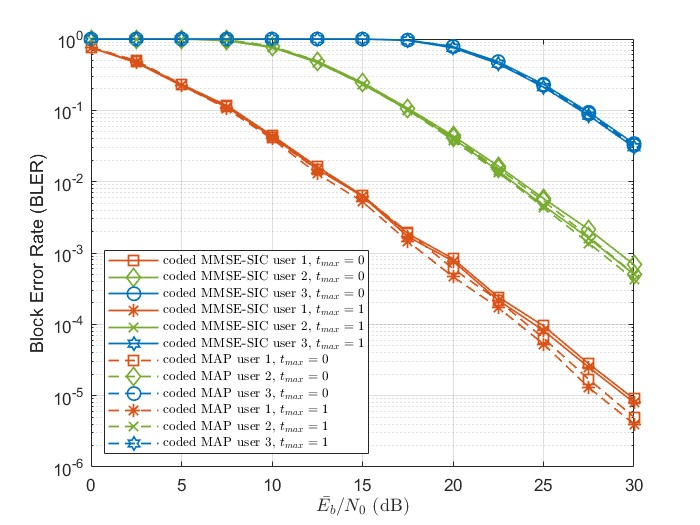
\includegraphics[width=0.9\linewidth]{figures/Chapter4/multi_resource_beta0.1_MMSESIC_BLER.jpg}
    \caption{BLER of MMSE-SIC-IDD and MAP-IDD with $R=2$, $(\beta_1,\beta_2,\beta_3)=(1,0.1,0.01)$, $t_{\max}=0$ and $t_{\max}=1$.}
    \label{fig:multi_resource_beta0.1_MMSESIC_BLER}
\end{figure}
\begin{figure}[htbp]
    \centering
    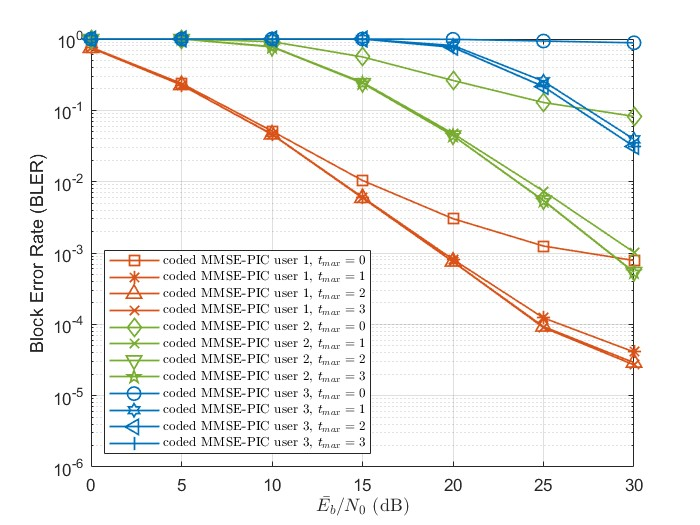
\includegraphics[width=0.9\linewidth]{figures/Chapter4/multi_resource_beta0.1_MMSEPIC_BLER.jpg}
    \caption{BLER of MMSE-PIC-IDD with $R=2$, $(\beta_1,\beta_2,\beta_3)=(1,0.1,0.01)$, $t_{\max}=0,1,2,3$}
    \label{fig:multi_resource_beta0.1_MMSEPIC_BLER}
\end{figure}
%\end{comment}

Figure.~\ref{fig:multi_resource_beta0.1_MMSESIC_BLER} shows the BLER performance of MMSE-SIC-IDD and MAP-IDD with unequal-$\beta_k$ case. 
Figure.~\ref{fig:multi_resource_beta0.1_MMSEPIC_BLER} shows the BLER performance of MMSE-PIC-IDD with unequal-$\beta_k$ case.
It's observed that MMSE-PIC-IDD strongly relies on reliable a priori information update because parallel cancellation relies directly on the a priori-based soft means of all interfering users. Compare with MMSE-SIC-IDD and MAP-IDD in figure.~\ref{fig:multi_resource_beta0.1_MMSESIC_BLER}, the performance is closed to all users, indicating that decoder-aided soft cancellation effectively reduces residual interference.

%\begin{comment}
\begin{figure}[htbp]
    \centering
    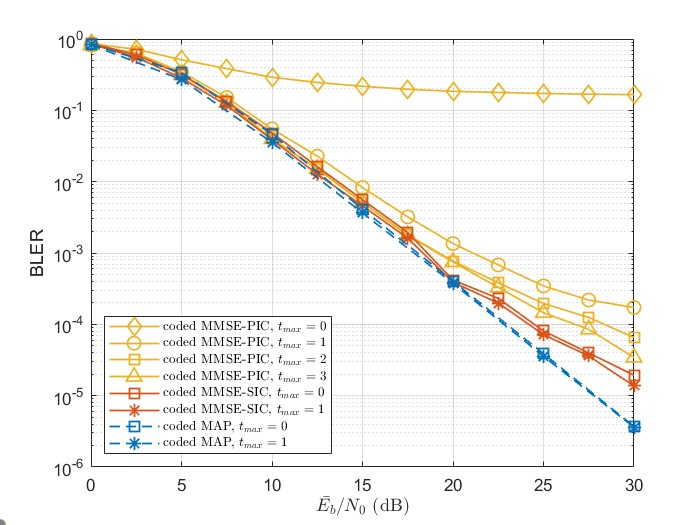
\includegraphics[width=0.9\linewidth]{figures/Chapter4/multi_resource_beta1_U3_BLER.jpg}
    \caption{BLER of different receiver structures with $R=2$, $U=3$ and $(\beta_1,\beta_2,\beta_3)=(1,1,1)$.}
    \label{fig:multi_resource_beta1_U3_BLER}
\end{figure}
%\end{comment}

Figure.~\ref{fig:multi_resource_beta1_U3_BLER} shows the BLER performance of MMSE-PIC-IDD, MMSE-SIC-IDD and MAP-IDD with equal-$\beta_k$ case.
For the MMSE-PIC-IDD scheme, convergence of the BLER is nearly achieved by $t_{\max}=3$. Consequently, the remaining simulations in this chapter are conducted solely using $t_{\max}=3$.
Compared with the MMSE-SIC-IDD and MAP-IDD, the performance is also closed, while MAP-IDD is slightly better in the high-SNR region.
It can also be observed that for both unequal-$\beta_k$ case and equal-$\beta_k$ case, the gain from increasing the value of $t$ is limited. This is due to the assumption of a block fading channel and the relatively moderate system loading.

%\begin{comment}
\begin{figure}[htbp]
    \centering
    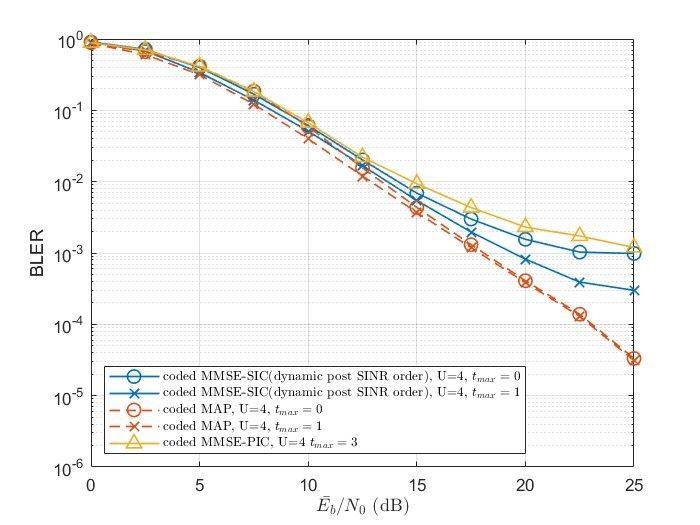
\includegraphics[width=0.9\linewidth]{figures/Chapter4/multi_resource_beta1_U4_BLER.jpg}
    \caption{BLER of different receiver structures with $R=2$, $U=4$ and $\beta_k=1$.}
    \label{fig:multi_resource_beta1_U4_BLER}
\end{figure}

\begin{figure}[htbp]
    \centering
    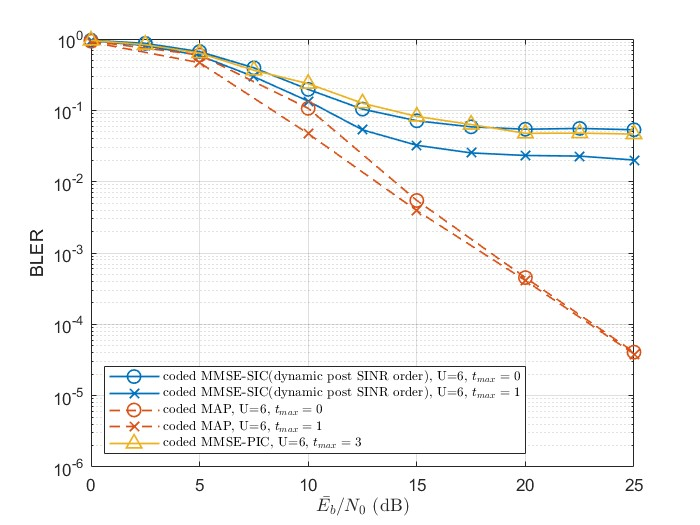
\includegraphics[width=0.9\linewidth]{figures/Chapter4/multi_resource_beta1_U6_BLER.jpg}
    \caption{BLER of different receiver structures with $R=2$, $U=6$ and $\beta_k=1$.}
    \label{fig:multi_resource_beta1_U6_BLER}
\end{figure}
%\end{comment}

Figure.~\ref{fig:multi_resource_beta1_U4_BLER} and ~\ref{fig:multi_resource_beta1_U6_BLER} are the case of 4-user and 6-user respectively. It can be seen that MAP-IDD maintains superior BLER performance owing to its near-optimal detection capability, whereas MMSE-based receivers becomes more sensitive to the increase in the number of user.




%\begin{comment}
\begin{figure}[htbp]
    \centering
    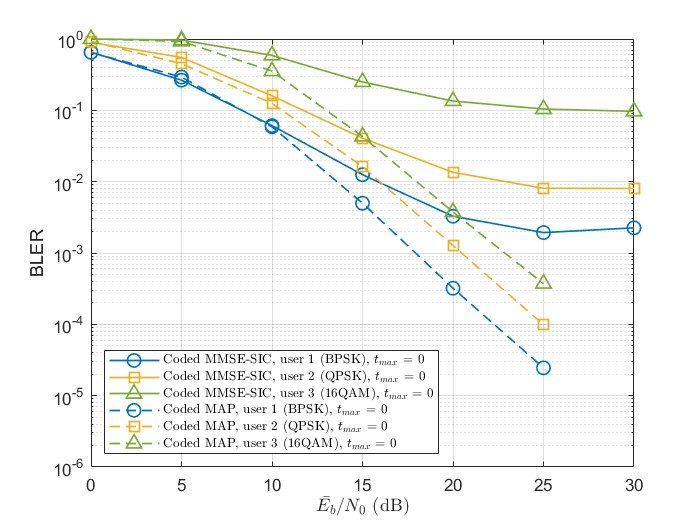
\includegraphics[width=0.9\linewidth]{figures/Chapter4/U3_BPSK_QPSK_16QAM_beta1_ite0.jpg}
    \caption{BLER of MMSE-SIC-IDD and MAP-IDD with $R=2$, $U=3$ and $\beta_k=1$. (BPSK, QPSK, 16QAM) is used. $t_{\max}=0$}
    \label{fig:U3_BPSK_QPSK_16QAM_beta1_ite0}
\end{figure}


\begin{figure}[htbp]
    \centering
    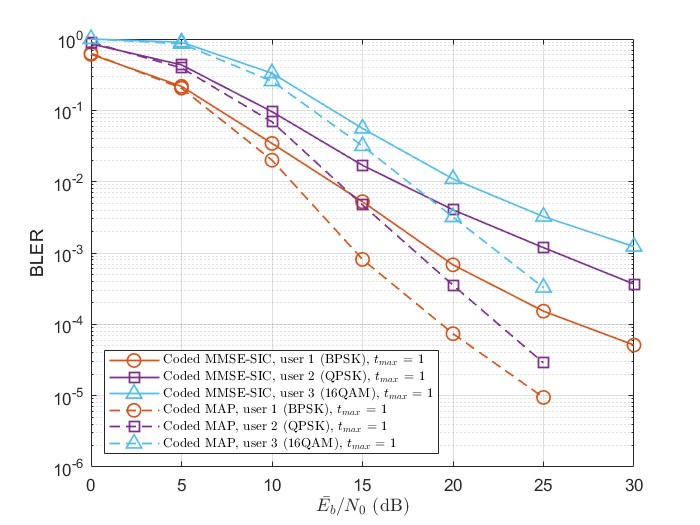
\includegraphics[width=0.9\linewidth]{figures/Chapter4/U3_BPSK_QPSK_16QAM_beta1_ite1.jpg}
    \caption{BLER of MMSE-SIC-IDD and MAP-IDD with $R=2$, $U=3$ and $\beta_k=1$. (BPSK, QPSK, 16QAM) is used. $t_{\max}=1$}
    \label{fig:U3_BPSK_QPSK_16QAM_beta1_ite1}
\end{figure}
%\end{comment}

Figure.~\ref{fig:U3_BPSK_QPSK_16QAM_beta1_ite0} and ~\ref{fig:U3_BPSK_QPSK_16QAM_beta1_ite1} consider three users using modulation (BPSK, QPSK, 16QAM). This two figures represent $t_{max}=0$ and $t_{max}=1$, respectively. 
Compare with BPSK modulation for every user, MAP-IDD can benefit from a priori information update even under block fading channel, since decoder feedback helps refine the APP weights of possible superimposed signals.


\section{Comparison and summary}

The simulation results show that the IDD is effective for coded multi-resource NOMA receivers, but the amount of gain depends on the detector type, system loading, and modulation order. For MAP-IDD, the detector already provides highly reliable soft information. Therefore, the additional gain from the a priori information update is smaller than that of the MMSE-based receivers in simple BPSK cases. However, MAP-IDD still achieves the best BLER performance in all simulated scenarios and remains robust when the number of users or modulation order~increases.

MMSE-SIC-IDD provides a favorable tradeoff between performance and complexity. By combining dynamic post-SINR ordering, variance-aware MMSE filtering, and decoder-aided cancellation, it can approach MAP-IDD in the three-user case and still performs well in the four-user case while BPSK modulation is used for every user. However, it is still based on linear filtering and sequential cancellation. When the system becomes heavily loaded, the  residual interference causes a clear performance floor.

MMSE-PIC-IDD has the advantage of parallel processing and lower receiver latency because all users can be detected simultaneously. However, its cancellation quality strongly depends on the reliability of the a priori information.


\chapter{Performance analysis of user pairing based on Channel quality indicator (CQI)}
\label{ch:CQI}
In this chapter, we will analyze the performance of user pairing based on Channel Quality Indicator (CQI) in a multi-user communication system. The CQI is a measure of the channel conditions experienced by a user and is used to optimize resource allocation and improve overall system performance. We will explore various user pairing strategies, evaluate their impact on system throughput, and discuss the trade-offs involved in selecting appropriate pairing schemes.

\section{Introduction of CQI}

\chapter{Conclusions and future work}
%% In chapter2
In chapter~\ref{ch:single-resource}, 


%% In chapter3
In chapter~\ref{ch:multi-resource}, 


%% In chapter4
In chapter~\ref{ch:coded}, 


%% In chapter5
In chapter~\ref{ch:cqi}, 

In future research, 
% 參考文獻
% References
\refmatter

% \bibliographystyle{abbrv}
\bibliographystyle{unsrt}

\bibliography{back/references}

% 附錄
% Appendices
% !TeX root = ../main.tex

\appendix{A}{Complete GDMA MUD Candidate Table}
\makeatletter
\def\@currentlabel{A}
\makeatother
\label{app:gdma-candidate-table}

\section{Complete GDMA Candidate MCS Combinations}

Table~\ref{tab:appendix-gdma-complete-candidates} lists the complete GDMA candidate MCS combinations simulated under the aggregate received-SNR definition in \eqref{eq:aggregate-received-snr}. Each entry gives the after-pair CQI state, the corresponding sum SE, and the required aggregate SNR such that all users satisfy $\mathrm{BLER}\leq 10^{-1}$. In Chapter~\ref{ch:cqi}, the dominated combinations are removed from this table to obtain the effective GDMA after-pairing states in Table~\ref{tab:gdma-states}.

\begin{table}[t]
\centering
\small
\caption{Complete GDMA after-pairing candidate states before removing dominated MCS combinations.}
\label{tab:appendix-gdma-complete-candidates}
\begin{tabular}{@{}ccc@{}}
\toprule
After-pair CQI state & Sum SE (bit/s/Hz) & Required $\Gamma^{\mathrm{agg}}_{\mathrm{th}}$ (dB) \\
\midrule
$(1,1)$ & 1.00 & 11.88 \\
$(1,2)$ & 1.17 & 14.02 \\
$(1,4)$ & 1.50 & 14.58 \\
$(1,5)$ & 1.83 & 15.53 \\
$(1,6)$ & 2.00 & 17.20 \\
$(1,7)$ & 2.50 & 22.31 \\
$(1,8)$ & 3.17 & 23.80 \\
$(1,9)$ & 3.50 & 24.42 \\
$(2,2)$ & 1.34 & 14.52 \\
$(2,4)$ & 1.67 & 16.94 \\
$(2,5)$ & 2.00 & 17.56 \\
$(2,6)$ & 2.17 & 18.27 \\
$(4,4)$ & 2.00 & 16.70 \\
$(4,5)$ & 2.33 & 19.56 \\
$(4,6)$ & 2.50 & 21.28 \\
$(5,5)$ & 2.66 & 20.02 \\
$(5,6)$ & 2.83 & 21.22 \\
$(6,6)$ & 3.00 & 21.62 \\
\bottomrule
\end{tabular}
\end{table}

% \input{back/appendix02}

\end{document}
